\documentclass[11pt,letterpaper,]{article}

\title{Design and Implementation of a Shelter Location-Allocation System in Calumpit, Bulacan}
\author{Calulo, Bryan Jett T., Cunanan, Lovely Angeline OL., Fabian, Elijah Inigo C.,}

\usepackage[T1]{fontenc}
\usepackage{uarial}
\renewcommand{\familydefault}{\sfdefault}
\usepackage{graphicx}
\usepackage{geometry}
	\geometry{margin=1in}
\usepackage{indentfirst}


\usepackage{titlesec}
\titleformat{\section}%
{\normalfont\normalsize\bfseries}%
{\thesection}%
{1em}%
{\MakeUppercase}
\titleformat{\subsection}%
{\normalfont\normalsize\bfseries}%
{\thesubsection}%
{1em}%
{}

\usepackage{fancyhdr}
\pagestyle{fancy}
\fancyhf{}
\fancyfoot[C]{\thepage}
\renewcommand{\headrulewidth}{0.0pt}

\usepackage{booktabs,longtable,threeparttable,siunitx,tabularx}
\usepackage{array,multicol,multirow,color,calc}
\newcolumntype{L}[1]{>{\raggedright\let\newline\\\arraybackslash\hspace{0pt}}p{#1}}
\newcolumntype{C}[1]{>{\centering\let\newline\\\arraybackslash\hspace{0pt}}p{#1}}
\newcolumntype{R}[1]{>{\raggedleft\let\newline\\\arraybackslash\hspace{0pt}}p{#1}}

\usepackage{caption}
\DeclareCaptionLabelSeparator*{spaced}{\\[1ex]}
\renewcommand{\thetable}{\arabic{table}}
\captionsetup[table]{
	%		font=sf,
	labelfont=bf,
	textfont=it, 
	format=plain,
	justification=justified,
	singlelinecheck=false,
	labelsep=spaced,skip=12pt
}
\captionsetup[figure]{
	%		font=sf,
	labelfont=bf,
	textfont=it, 
	format=plain,
	justification=justified,
	singlelinecheck=false,
	labelsep=spaced,skip=12pt
}
\usepackage[american]{babel}
\usepackage{csquotes}
\usepackage[style=apa,defernumbers=true]{biblatex}
\DeclareLanguageMapping{american}{american-apa}

\usepackage{etoolbox}

\AtBeginEnvironment{tabular}{\small\sffamily}
\AtBeginEnvironment{tabularx}{\small\sffamily}
\AtBeginEnvironment{abstract}{\bfseries}

\setlength{\headheight}{14.5pt}
\setlength{\headsep}{14pt}

\usepackage[shortcuts]{extdash}
\pretolerance=5000
\tolerance=9000 
\emergencystretch=10pt
\addbibresource{reference.bib} %filename of your .bib database
\graphicspath{{Figures/}}	%change graphic path folder
\usepackage{lipsum} %for dummy text

\usepackage{setspace}
\usepackage{amsmath, amssymb, float, subcaption}

\begin{document}

{\centering{\large\bfseries
	\MakeUppercase{Design and Implementation of a Shelter Location- 
		\protect\\Allocation System in Calumpit, Bulacan}
	}
	
	\vspace{6pt}
	
	Bryan Jett T. Calulo, Lovely Angeline OL. Cunanan, and Elijah Iñigo C. Fabian
	
	\vspace{6pt}
	
	Bulacan State University
	
\par}


\begin{abstract}
	The Philippines, being highly vulnerable to disasters such as typhoons and floods, ranks first in the World Risk Index. Among the municipalities of Bulacan, Calumpit is particularly prone to severe flooding. Furthermore, the current evacuation system faces challenges such as overcrowding and inefficient resource use. While mathematical models can optimize shelter allocation, they are often inaccessible to decision-makers without mathematical expertise. To address this, a data-driven decision support system was developed. Shelter Location-Allocation System identifies suitable shelters and assigns communities in an optimal manner. The system integrates the Bilevel No Transfer (BNT) model, considering distance, cost, capacity, and shelter hierarchy, and applies a genetic algorithm to determine the best allocation strategy. All parameters and data are fully customizable, allowing decision-makers to tailor the system to their needs. The system was evaluated by end-users and IT experts, receiving high acceptability scores, with mean ratings greater than 9.0 across all criteria. These results indicate the system’s quality in supporting data-driven disaster response planning, offering a scalable solution for improving evacuation strategies in flood-prone areas.
	
	\vspace{6pt}
	\noindent Key Words: \normalfont Shelter Optimization, Disaster Planning, Location Allocation
\end{abstract}

\onehalfspacing

\section{Introduction}
	The Philippines experiences typhoons, earthquakes, and volcanic eruptions each year, leaving people vulnerable and displaced as the country is situated within the Pacific Ring of Fire and directly in the path of the typhoon belt in the Pacific Ocean. For instance, typhoon Haiyan, better known as Super Typhoon Yolanda devastated the nation in 2013 and displaced over 4 million people, exposing severe shortcomings in the Philippine shelter allocation systems \parencite{Iuchi2019}, highlighting the urgent need for efficient and responsive disaster management strategies. Despite ongoing efforts, the country continues to face significant challenges in shelter allocation, such as overcrowding, resource distribution inefficiency, and poor accessibility.
	
	Overcrowding remains a persistent issue, with many shelters operating beyond intended capacity. Accessibility problems further worsen the situation, as shelters are often located at distances difficult for affected individuals, particularly those in rural or remote areas, to reach due to poor infrastructure. Compounding these issues such as disaster preparedness teams not using data-driven decision-making increases the likelihood of making incorrect decisions, highlighting the data and planning gaps that hinder effective decision making and timely shelter assignments. This emphasizes the need to develop innovative approaches to improve shelter allocation in disaster preparedness.
	The concept of shelter allocation has been a critical aspect of disaster management throughout history, when communities would seek refuge in caves or fortified structures during emergencies. After World War II, air raid shelters established in urban areas evolved in response to natural disasters, and humanitarian efforts developed temporary shelters for displaced populations.
	
	Shelter allocation refers to the process of assigning displaced communities to available shelters during disasters \parencite{Yin2023}. While shelter location-allocation focuses on determining locations where shelters would be constructed, to then be used for the displaced population \parencite{Xiujuan2019}. These processes are crucial to disaster prevention and mitigation, ensuring the safety and well-being of affected populations by providing secure accessible, and adequate temporary shelters. Effective shelter allocation involves considerations such as shelter capacity, proximity to disaster sites, and the specific needs of vulnerable communities.
	
	This study proposes a data-driven solution ensuring an effective and feasible implementation of shelter allocation. This would be by developing a decision support system using a genetic algorithm (GA), to address the inefficiencies in shelter allocation. GA optimizes solutions by mimicking the process of evolution such as selection, crossover, and mutation, to identify an optimal outcome. In shelter allocation, GA can optimize the assignment process by simultaneously considering factors such as shelter capacity, location, and accessibility. This approach aims to minimize overcrowding, improve resource distribution, and enhance overall efficiency in managing shelters during disasters.
	
	Given the Philippines’ frequent exposure to natural disasters, implementation of a shelter allocation system is essential. Calumpit, Bulacan was chosen for its high vulnerability to flooding since it has been a catch basin for neighboring areas. Despite the multitude of studies formulating models to address the shelter location-allocation problem, there remains a clear lack of system integration. This gap makes it difficult for decision-makers, particularly those unfamiliar with the mathematical models proposed in several studies, to apply them effectively in their decisions. This study is dedicated to the development of a programmed system that uses genetic algorithm to address the challenges experienced in the Philippines, focusing on Calumpit, Bulacan. The proposed shelter location-allocation system has the potential to significantly improve disaster response efficiency and enhance safety for displaced individuals. The insights from this study may be applied to other municipalities facing similar challenges, contributing to the national effort to strengthen disaster resilience.
	
	This thesis’s objective is to create a shelter allocation system using Genetic Algorithm and the Bilevel No Transfer model to create an optimal strategy for evacuation in Calumpit. Data was gathered from Calumpit’s LGU to create an accurate representation of the municipality.
	

\section{Methods}

This chapter outlines and expands upon the research methodology for the
design and implementation of a shelter location-allocation system using a genetic
algorithm for the optimization of shelter placement in disaster-prone areas. This
methodology provides a systematic approach for a clear framework for system
design, model implementation, and evaluation.
	
	\subsection{Research Design}
	
	The research design for this study is mixed method applied research, this approach combines both quantitative and qualitative methods to provide a structured framework for development and evaluation of the shelter location allocation system
	The applied research aspect of the study aims to deliver a functional and reliable shelter location-allocation system that disaster response agencies can easily deploy and adapt. The quantitative research of this study aims to measure and analyze the acceptability of the proposed system using TAM determinants and the ISO/IEC 25010 standard. The qualitative research of this study is to understand the current issues of shelter location-allocation from the stakeholders’ perspectives.
	
	\subsection{Model Adoption}
	
	The study adopted a model called the Bilevel No-Transfer (BNT) model, which solves the shelter location-allocation problem under disaster scenarios. Discussed in a published paper by \textcite{LeahUP}, the model is effective when assigning communities to shelters without allowing transfers between different shelter levels during recovery. Once assigned to a shelter in the BNT model, evacuees remain in that shelter until the disaster subsides, eliminating the need for transfers between shelters. The objective function for the BNT model can be expressed as follows:
	
	Minimize 
	\begin{equation}
		wt_{dist}\sum_{j=1}^{N}\sum_{i=1}^{M}d_{ij}P_{i}x_{ij}+wt_{cost}\sum_{k=1}^{2}\sum_{j=1}^{N}C_{j}^{(k)}y_{j}^{(k)} 
	\end{equation}
	
	The constraints of the model include the distance, capacity, assignment, and binary constraints, each playing a role in ensuring the model functions effectively under the disaster response scenario. Equations for these constraints are shown below:
	
	\textit{Distance Constraint.} Equation \ref{c1} ensures that each community is allocated to a shelter within a defined maximum distance. 
	
	\begin{equation} 	
		\label{c1}
		d_{ij}x_{ij} \le D_{i}, \forall i = 1,..., M,  \forall j = 1,..., N 
	\end{equation}
	
	\textit{Capacity Constraint.} Equation \ref{c2} guarantees that the total number of evacuees assigned to a shelter does not exceed its maximum capacity. 
	
	\begin{equation} 
		\label{c2}
		\sum_{i=1}^{M}LP_{i}x_{ij} \le \sum_{k} Area_{j}^{(k)} y_{j}^{(k)}, \forall j = 1,..., N , k=1,2
	\end{equation}
	
	\textit{Assignment Constraints.} Equations \ref{c3} and \ref{c4} ensures that the total assigned shelters and level 2 shelter does not exceeds over the user defined parameters respectively.  Equation \ref{c5} ensures that every community is assigned to exactly one shelter. Equation \ref{c6} ensures that the assigned shelter does not duplicate like being opened as level 1 and level 2 at the same time. This prevents problems in shelter allocation and ensures that each community has a designated place.
	
	\begin{equation} 
		\label{c3}
		\sum_{k=1}^{2} \sum_j={1}^{N}y_{j}^{(k)} \le MaxSh
	\end{equation}
	\begin{equation}
		\label{c4} 
		\sum_j={1}^{N}y_{j}^2 \le MaxL2
	\end{equation}
	\begin{equation}
		\label{c5}
		\sum_{j=1}^{N}x_{ij} = 1, \forall i=1,...,M
	\end{equation}
	\begin{equation}
		\label{c6}
		\sum_{k=1}^{N}y_{j}^{(k)} \le 1, \forall j=1,...,N
	\end{equation}
	
	\textit{Binary Constraint.} This constraint ensures that the model only takes binary variable, where can either be true (1) or false (0).
	
	\begin{equation}
		\label{c7}
		x_{ij}, y_{j}^{(1)},y_{j}^{(2)} \in \{0,1\}, \forall i=1,...,M,  \forall j=1,...,N
	\end{equation}
	
	\noindent Where:
	\\$wt_{dist}$ – weight given to the distance cost.
	\\$wt_{cost}$ – weight given to the fixed shelter cost.
	\\$M$ – total number of communities.
	\\$N$ – total number of potential shelter locations.
	\\$d_{ij}$ – distance between shelter i and community j.
	\\$P_{i}$ – population of the community i.
	\\$C_{j}^{(k)}$ – fixed cost for establishing shelter j of level k.
	\\$x_{ij}$ – binary decision variable indicating if community j is assigned to shelter i.
	\\$y_{j}^{(k)}$ – binary decision variable indicating if shelter j of level k is opened.
	\\$L$ - area allotted per individual
	\\$D_{i}$ – maximum distance that community i can be traveled.
	\\$Area_{j}^{(k)}$ - area of shelter j of level k.
	\\$MaxL2$ - maximum number of level 2 shelters to be opened.
	\\$MaxSh$ - maximum number of shelters to be opened.
	\\
	
	Checking if a solution exists based on the user defined parameters is a must in developing the system thus conducting feasibility checks before executing the algorithm. This adds a feature that allows users to view if their inputs are incorrect having an additional functionality and capability of the system.
	
	The following conditions should satisfy else no solution exists:
	
	\begin{equation} 
		\label{f1}
		Area_{j}^{(2)} \ge Area_{j}^{(1)}, \forall j = 1, ..., N
	\end{equation}
	
	Condition \ref{f1} checks if shelter j area for level 2 is greater than or equal to their area for level 1. 
	
	\begin{equation} 
		\label{f2}
		MaxL2 \le MaxSh
	\end{equation}
	
	Condition \ref{f2} checks if the user defined number of maximum level 2 shelters is less than to number of maximum shelters.
	
	\begin{equation} 
		\label{f3}
		\exists j \in d_{ij} \le D_{i}, \forall i = 1, ..., M
	\end{equation}
	
	Condition \ref{f3} checks if there exists a distance from community i to all shelters that is less than or equal to its max distance.
	
	\begin{equation} 
		\label{f4}
		\exists i \in LP_{i} \le Area_{j}^{(2)}, \forall j = 1, ..., N
	\end{equation}
	
	Condition \ref{f4} checks if there exists a level 2 shelter that could accommodate a community i by their population multiplied by the area allotted per individual. 
	
	\begin{equation} 
		\label{f5}
		\sum_{i=1}^{M}P_{i} \le L\sum_{j=1}^{N}Area_{j}, \forall i=1,...,M,  \forall j=1,...,N
	\end{equation}
	
	Condition \ref{f5} checks if the total population is less than or equal to the total area of shelters multiplied to area allotted per individual. If this fails, then it is theoretically impossible to allocate all individuals given with their shorted capacity of shelters.
	
	The penalty function was used to handle the problem constraints. Instead of discarding infeasible solutions or chromosomes, they are assigned a very large objective value making them not fit to be a solution. The type of penalty to be used is the Courant-Beltrami penalty function method, as shown in equation \ref{p1}.
	
	\begin{equation} 
		\label{p1}
		h(x)=(g^+(x))^2
	\end{equation}
	
	where
	
	\begin{equation} 
		\label{p2}
		g^+(x)=max\{g(x),0\}
	\end{equation}
	
	where $g(x)$ is a constraint function of the form $g(x)\le0$. 
	\\
	The new objective function would be adding the initial objective value $f(x)$ to the penalty multiplied by some constant $\gamma$ as shown in equation \ref{p3}.
	
	\begin{equation} 
		\label{p3}
		f_{new}(x)=f(x)+\gamma\sum_{i=1}^{n}(max\{g_i(x),0\})^2
	\end{equation}
	
	where $g_1(x),g_2(x),...g_n(x)$ are the constraints of the model of the form $g_i(x)\le0$, and $\gamma\in\mathbb{R}^+$ is sufficiently large, where for this thesis is set to $10^{20}$. The penalty would add up to the objective value for each constraints it violated, otherwise it would not affect the objective value.	
	
	In a study created by \textcite{Mathew2012}, Genetic Algorithms are based on the concept of natural selection and evolves possible solutions through selection, crossover, and mutation. The algorithm iteratively evolved a population of potential solutions, gradually converging toward an optimal solution. The BNT model was solved using Integer-based Genetic Algorithm implemented in Python. This decision satisfies the assignment constraint of the model, and with Python being a well suited programming language for both data simulation and system development. For this study, the selection, crossover, and mutation used are roulette wheel, uniform, and random reset respectively.
	
	\subsection{Process of Developing the System}
	
	The study employed a structured system development methodology following the Agile approach, chosen for its flexibility and iterative nature, allowing for continuous refinement and adaptation of the system based on feedback and results. Development includes regular reviews and adjustments to ensure the system evolves effectively to meet technical and user needs. 
	
	\begin{figure}[h!]
		\caption{A representation of an Agile approach}
		\centering
		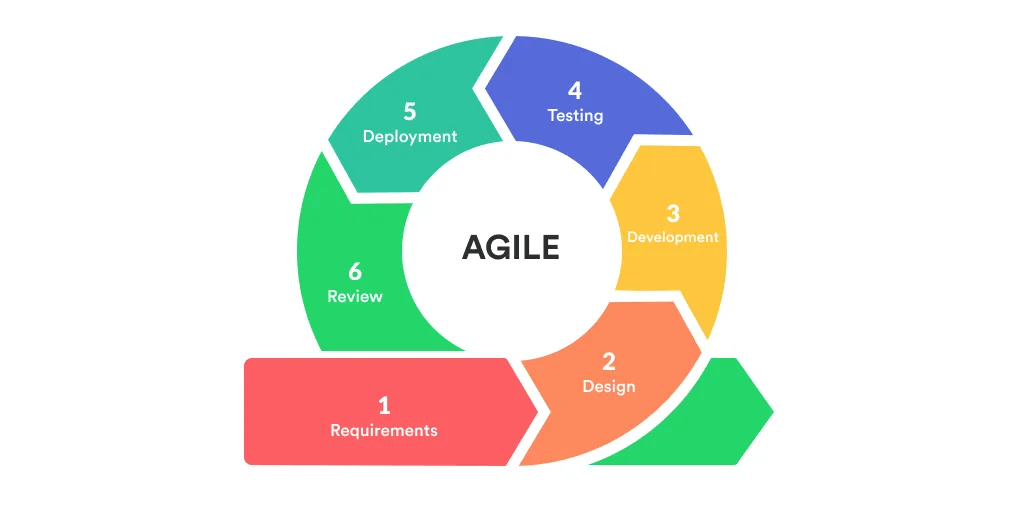
\includegraphics[width=0.9\columnwidth]{AGILE}
		\label{Agile}
	\end{figure}
	
	The researchers followed the Agile approach in several phases as shown in figure \ref{Agile} by \textcite{Jayathilaka2020}. Firstly, during the requirement analysis phase, researchers gathered comprehensive information about the system requirements by reviewing relevant literature that pertains to the thesis. Moreover, an interview with the client was conducted to find out more about the current issues LGUs are facing regarding evacuation. This phase ensures that all necessary features are identifed and prioritized based on their importance.
	
	\begin{figure}[h!]
		\caption{System Architecture}
		\centering
		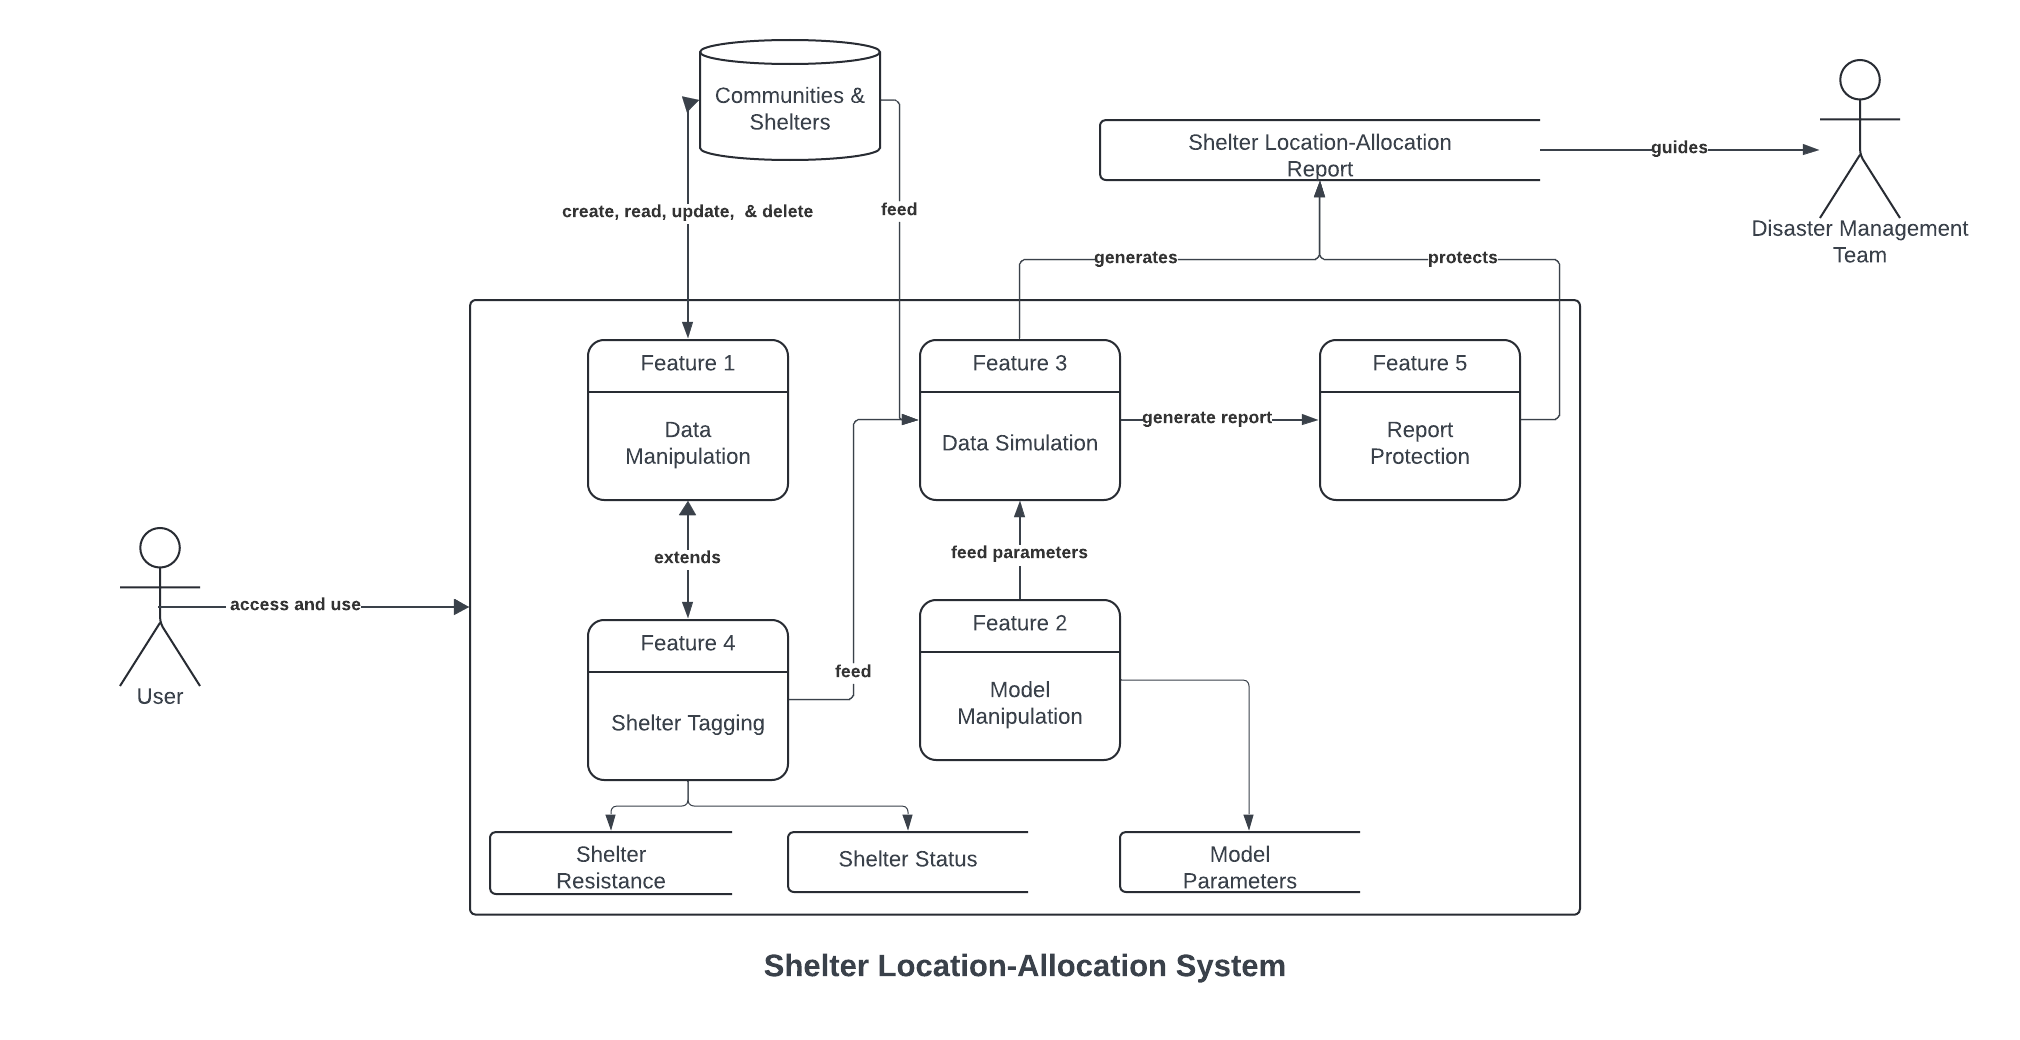
\includegraphics[width=0.75\columnwidth]{Context Diagram}
		\label{SystemArch}
	\end{figure}
	Figure \ref{SystemArch} the interaction of two actors, the user of the system and disaster management team. The community and shelter data will be fed into a system which features data manipulation and shelter tagging. With the cleaned and finished data, data simulations may begin together with the model parameters specified by the users. Lastly, a report will be generated and can be password-protected. The report will be used by the disaster management team as guidance for decision making in allocation of residents to the correct shelter.
	
	\begin{figure}[h!]
		\caption{The ERD Schema}
		\centering
		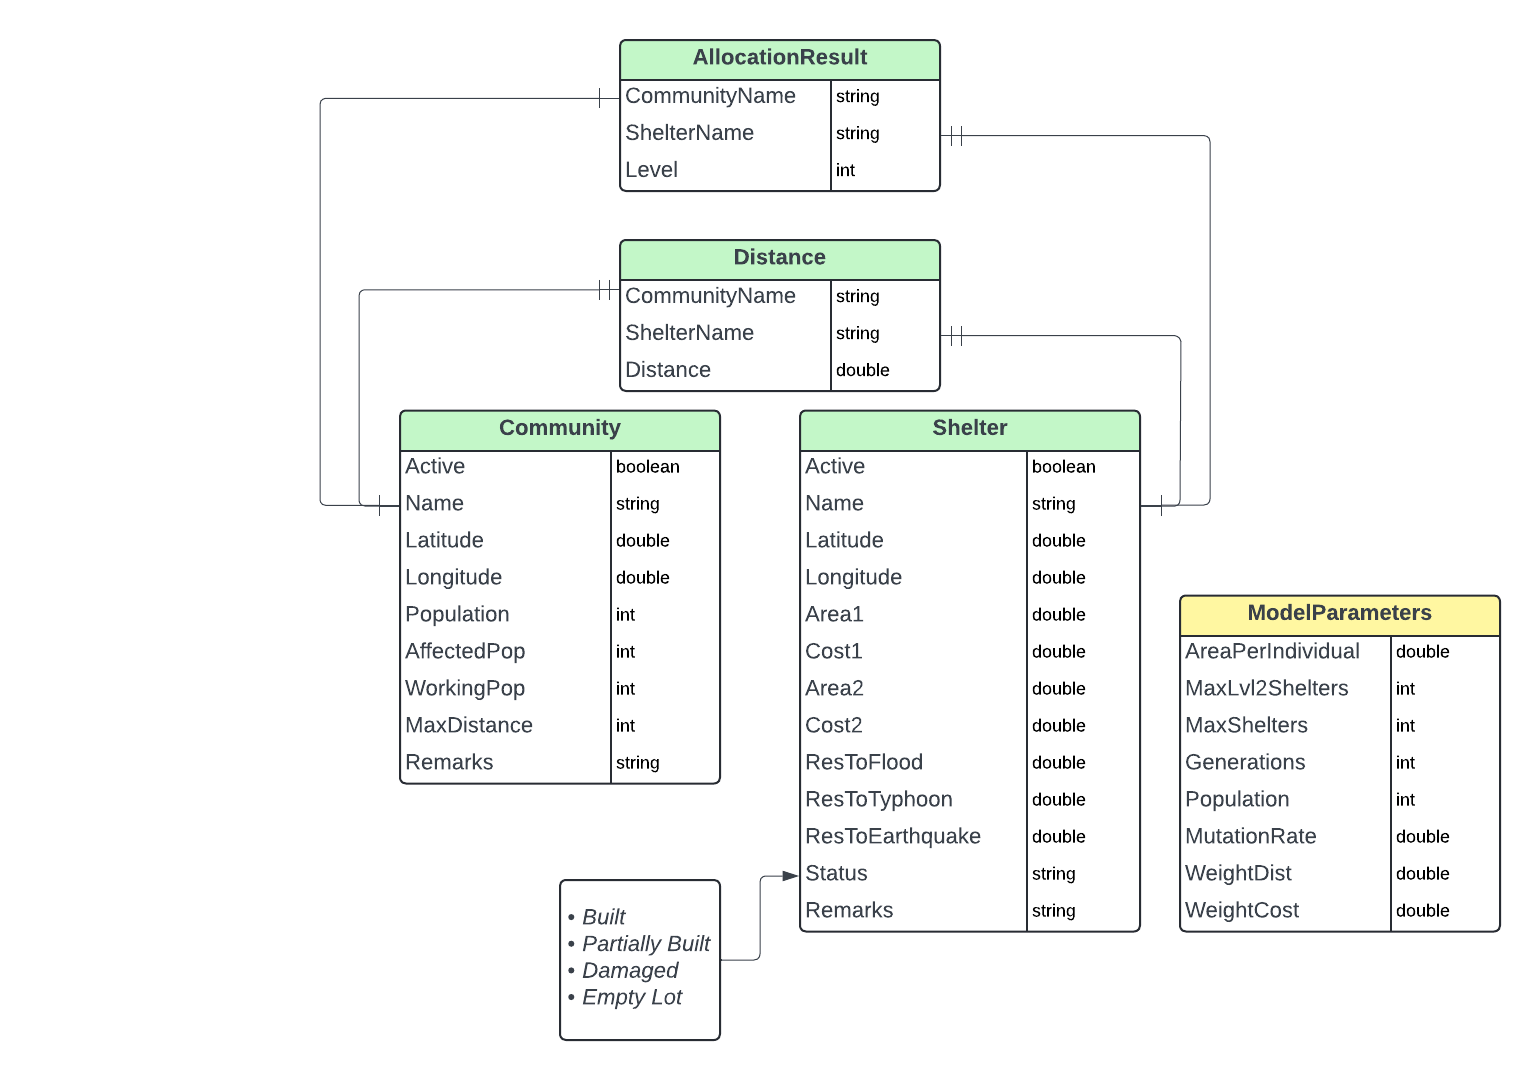
\includegraphics[width=0.6\columnwidth]{ERD}
		\label{ERD}
	\end{figure}
	Figure \ref{ERD} shows the entity relationship (ERD) which contains 4 entities, Community, Shelter, Distance, and ModelParameters. Distances are derived from the locations of Shelter and Community, then saved accordingly to be used in performing the system’s model. ModelParameters saves the current settings for the model and algorithm.
	
	The system was developed using the Python programming language, and Qt framework to efficiently implement the graphical user interface (GUI) of the system. Visual Studio Code was utilized as the integrated development environment (IDE), and QtDesigner as an extension for creating frontend designs through the Qt framework.
	Developing the system using Python allows the use of Python libraries. These include PySide6 which is responsible for the GUI that uses the Qt framework, Pandas and openpyxl for handling data, Folium, OSMnx, network, and scikit-learn for displaying and calculating the map shown in the system. Numpy is used for executing genetic algorithm. Additionally, msoffcrypto-tool and XlsxWriter are used for report protect and lastly, pyinstaller for building the system.
	
	
	\subsection{System Evaluation}
	
	The target population of this study consists of 23 end-users and 5 IT experts. For end-users, the MDRRMO and MSWDO of the municipality of Calumpit, meanwhile for IT experts include CICT professors from Bulacan State University, as well as those in careers related to developing a system. The diversity of perspective of these are important for the evaluation of the system’s acceptability.
	
	The system was evaluated by preparing and distributing survey questions based on the TAM and ISO/IEC 25010 to target samples respectively. The questionnaires are a 10-point numerical scale survey and verbally interpreted based from \textcite{Eladia2024} This ensured that the developed system acquires feedback from potential users as well as from experts in software engineering and development.
	
	\subsection{System Preliminaries}
	
	Interviews was conducted with representatives from local government units (LGUs) specifically from the target population to understand their existing shelter allocation process, challenges, and expectations for a decision support system. The gathered information has undergone several stages. This ensures it meets the needs of the system and allows for an accurate assessment of its effectiveness.
	
	Table \ref{dataSource} presents all the data variables on communities and shelters used in the model, along with their respective sources. Researches added empty lots across Calumpit to be appended to shelter data as shown in table \ref{AppendData}. These lots are identified and selected to be resistant to hazards, specifically floods with the assistance of Nationwide Operational Assessment of Hazards (NOAH) website. 
	\begin{table}[H]
		\centering
		\caption{Variables, Descriptions, and Sources for Community and Shelter Data}
		\label{dataSource}
		\resizebox{\columnwidth}{!}{
			\begin{tabular}{|c|p{0.2\columnwidth}|p{0.4\columnwidth}|}
				\hline
				\textbf{Variable} & \textbf{Source} & \textbf{Description} \\ \hline
				\multicolumn{3}{|c|}{\textit{\textbf{Community}}}\\ \hline
				Name & LGU interview & Identity of a community \\ \hline
				Longitude & Google Map \& LGU interview & Longitudinal coordinates \\ \hline
				Latitude & Google Map \& LGU interview & Latitudinal coordinates \\ \hline
				Population & Philippine Atlas (2020 population) & Number of individuals living in a community \\ \hline
				AffectedPop & Assumed 12\% of Population & Number of individuals affected during a disaster \\ \hline
				MaxDistance & Maximum distance generated in distance calculation & Distance allowed to travel by a community \\ \hline
				\multicolumn{3}{|c|}{\textit{\textbf{Shelter}}} \\ \hline
				Name & LGU interview & Identity of a shelter \\ \hline
				Longitude & Google Map \& LGU interview & Longitudinal coordinates \\ \hline
				Latitude & Google Map \& LGU interview & Latitudinal coordinates \\ \hline
				Area1 & Google Map & Lot area of a shelter (level 1) \\ \hline
				Cost1 & Assumed 7,700 * Area1 & Cost for constructing/maintaining a shelter with Area1 \\ \hline
				Area2 & Assumed Area1 * 2 & Lot area of a shelter (level 2) \\ \hline
				Cost2 & Assumed 60,000 * Area1 & Cost for constructing/maintaining a shelter with Area2 \\ \hline
				ResToFlood & LGU interview & Resistance to flood indicator \\ \hline
				ResToTyphoon & LGU interview & Resistance to typhoon indicator \\ \hline
				ResToEarthquake & LGU interview & Resistance to earthquake indicator \\ \hline
				Status & LGU interview & State of the physical structure of a shelter indicator \\ \hline
				\multicolumn{3}{|c|}{\textit{\textbf{Distance between Community and Shelter}}} \\ \hline
				distance & OpenStreetMap API & distance needed to travel by a community to a shelter  \\ \hline
			\end{tabular}
		}
	\end{table}
	
	
	
	\begin{table}[H]
		\centering
		\caption{Sources of Appended Shelter Data}
		\label{AppendData}
		\resizebox{0.6\columnwidth}{!}{
			\begin{tabular}{|c|c|}
				\hline
				\multicolumn{1}{|c|}{\textbf{Variable}} & 
				\multicolumn{1}{c|}{\textbf{Source}} \\ \hline
				Cost1     & Assumed Area1 * (60,000 + 12,500) \\ \hline
				Cost2     & Assumed (Area2 * 60,000) + (Area1 * 12,500) \\ \hline
				ResToFlood     & Assumed TRUE \\ \hline
				ResToTyphoon    & Assumed TRUE \\ \hline
				ResToEarthquake     & Assumed TRUE \\ \hline
				Status     & Already an Empty Lot \\ \hline
				
			\end{tabular}
		}
	\end{table}


\section{Results and Discussion}
 This chapter details the functionalities of the developed system. Moreover, the system answers the optimal shelter
location-allocation for Calumpit, and presents the evaluation results.

	\subsection{The Developed System}
	The researchers and developers developed a decision support system to optimize shelter location allocation since there was a lack of system development. Identifying the most optimal shelter facility for a community is the system's main function. Specifically, it has five key features.
	
	Data Modification is the process of creating, updating, or deleting data within the system to maintain accuracy and relevance. Figures \ref{db}, \ref{commMan}, and \ref{shelMan} show parts on system with this feature.
	
	\begin{figure}[H]
		\centering
		\caption{Data Modification UI}
		
		\begin{subfigure}{0.4\textwidth}
			\caption{Dashboard}
			\label{db}
			\centering
			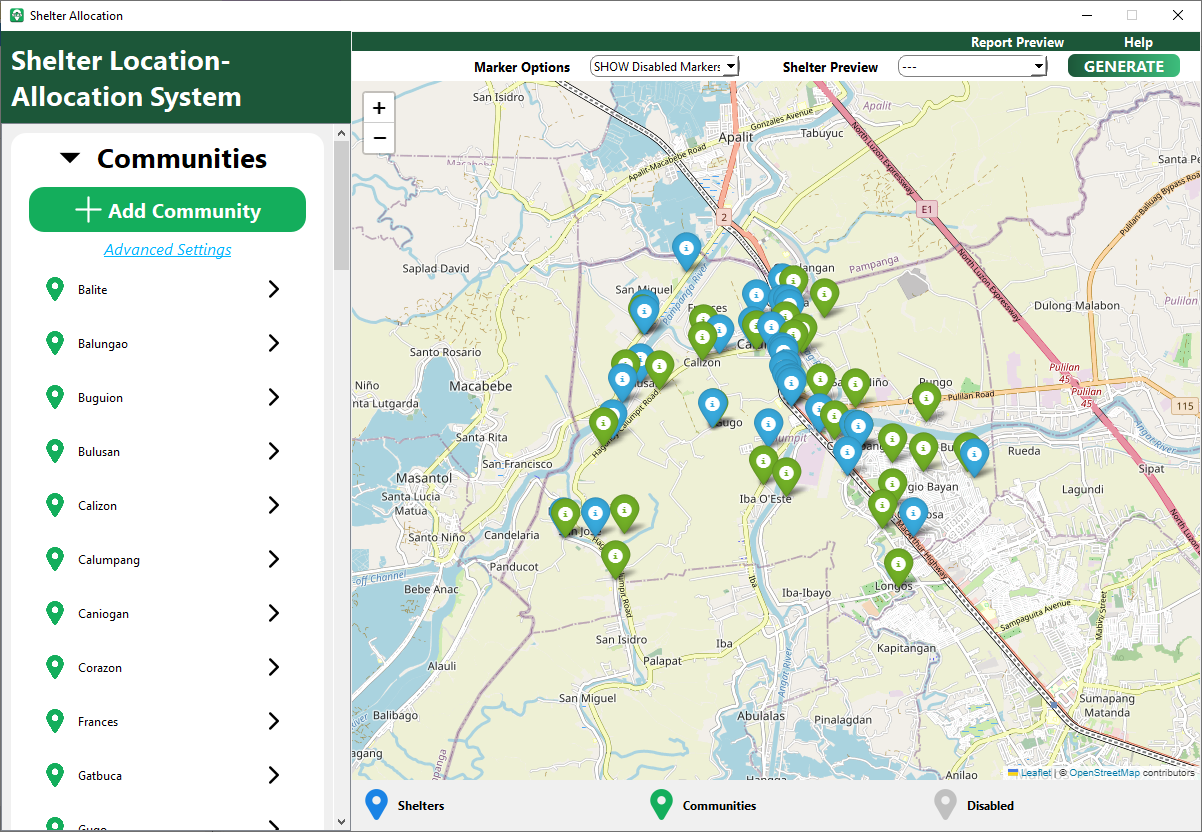
\includegraphics[width=\linewidth]{Chapter 4/dashboard}
		\end{subfigure}
		
		\vspace{0.1cm}
		\begin{subfigure}{0.3\textwidth}
			\caption{Community Management}
			\label{commMan}
			\centering
			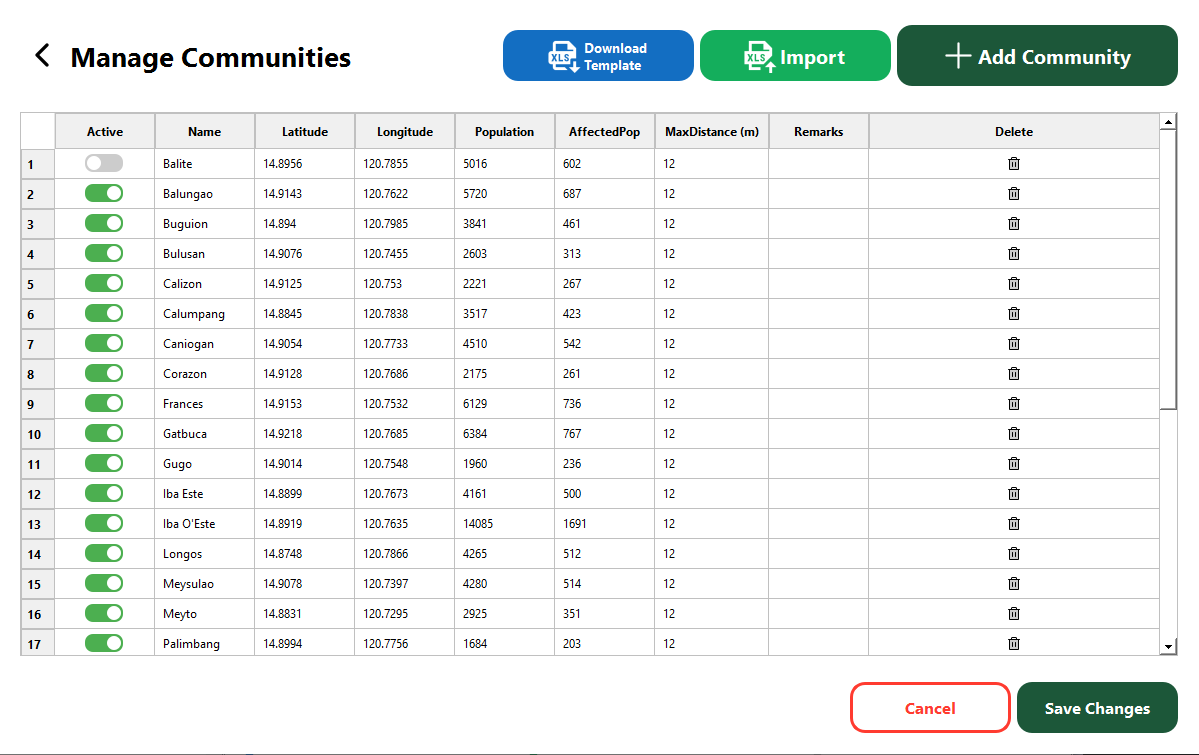
\includegraphics[width=\linewidth]{Chapter 4/commadvanced}
		\end{subfigure}
		\hspace{0.5cm}
		\begin{subfigure}{0.3\textwidth}
			\caption{Shelter Management}
			\label{shelMan}
			\centering
			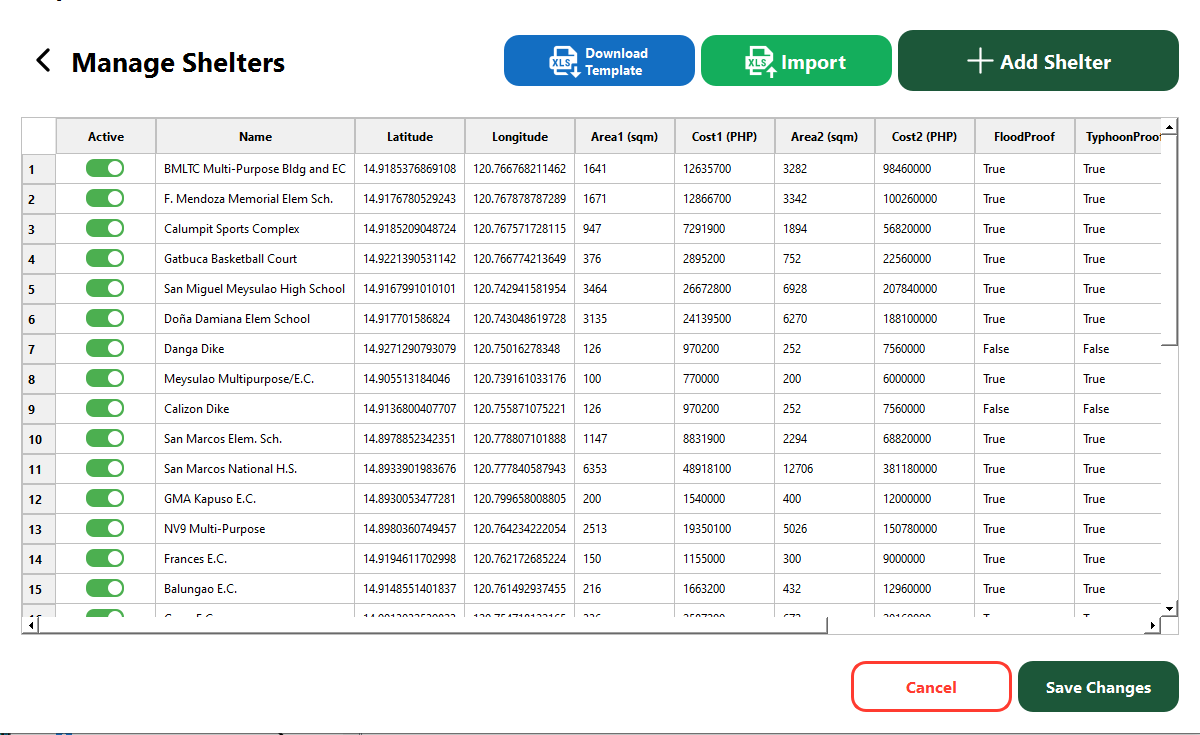
\includegraphics[width=\linewidth]{Chapter 4/sheladvanced}
		\end{subfigure}
		
	\end{figure}
	

	
	Model Modification concerns the parameters to be used in the model that may be modified for a more ideal setup depending on the preferences of the user.   Figure \ref{modelSet} shows part on system with this feature.
	
	\begin{figure}[h!]
		\caption{Model Parameter Settings}
		\centering
		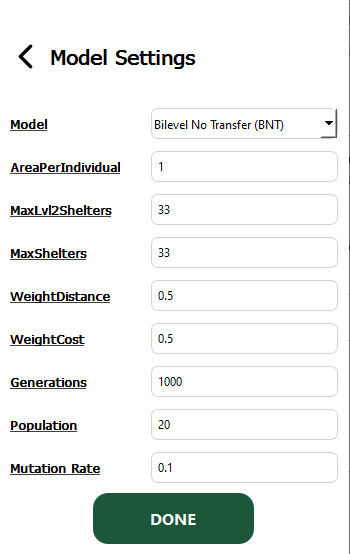
\includegraphics[width=0.3\columnwidth]{Chapter 4/modelsettings}
		\label{modelSet}
	\end{figure}
	
	Data Simulation pertains to solving the model by running the Genetic Algorithm, which then generates and displays the best allocation of the municipality. Figures \ref{solveProg}, and \ref{shelAllocRep} show parts on system with this feature.
	
	\begin{figure}[h!]
		\centering
		\caption{Data Simulation UI}
		
		\begin{subfigure}{0.45\textwidth}
			\caption{Progress Dialog}
			\centering
			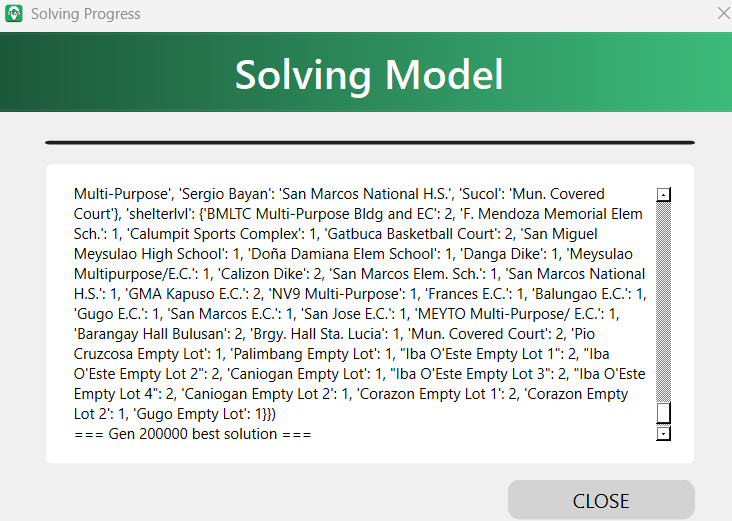
\includegraphics[width=\textwidth]{Chapter 4/progress}
			\label{solveProg}
		\end{subfigure}
		\hspace{0.5cm}
		\begin{subfigure}{0.45\textwidth}
			\caption{Report Dialog}
			\centering
			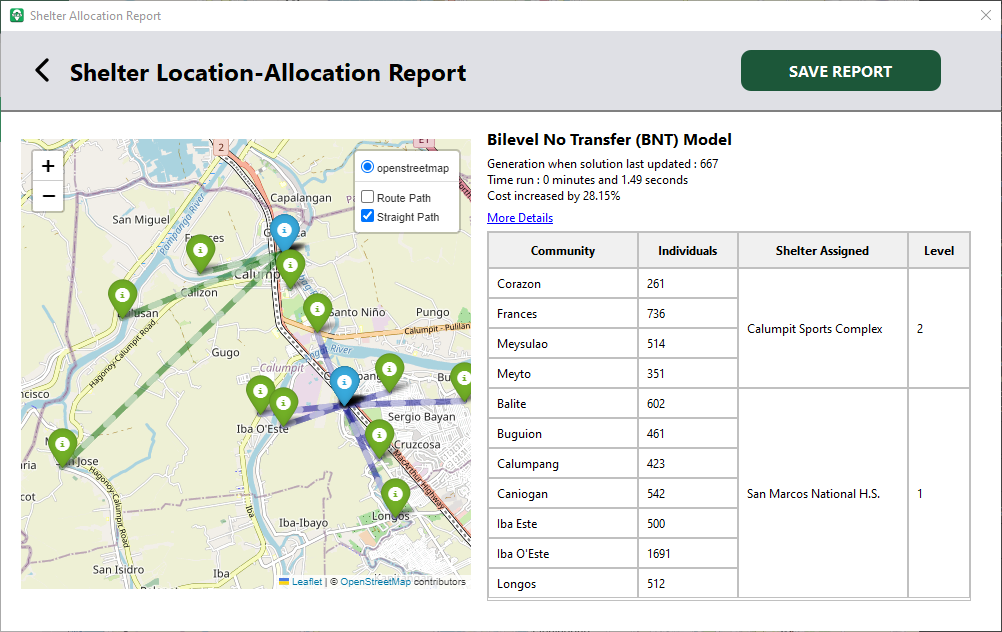
\includegraphics[width=\textwidth]{Chapter 4/alloc report}
			\label{shelAllocRep}
		\end{subfigure}
		
	\end{figure}
	
	Shelter Tagging concerns the classification of shelters based on both structural resilience and current condition, ensuring shelters are appropriately assigned to communities based on availability, cost, and risk levels. Figure \ref{solveSet} shows part on system with this feature.
	
	\begin{figure}[h!]
		\caption{Solve Settings}
		\centering
		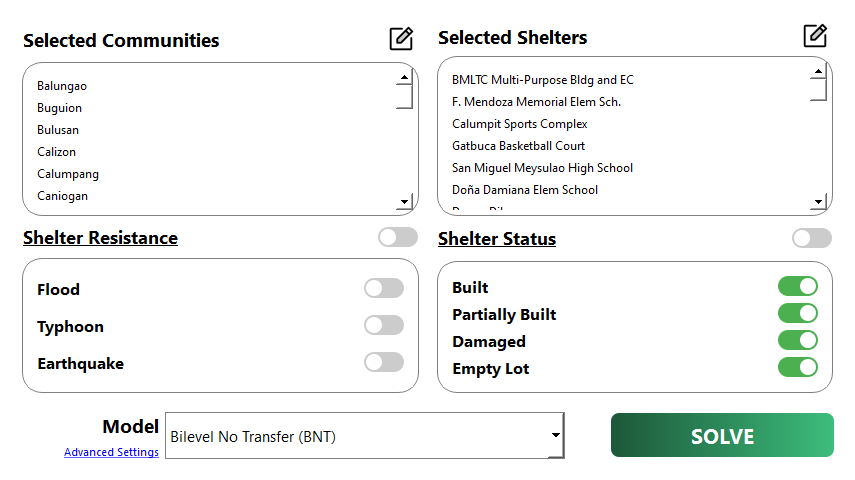
\includegraphics[width=0.6\columnwidth]{Chapter 4/solvesettings}
		\label{solveSet}
	\end{figure}
	
	To maintain confidentiality and prevent the unauthorized modification of reports, a Report Protection has been implemented in the system. Figure \ref{passPop} shows part on system with this feature.
	
	\begin{figure}[h!]
		\caption{Input Password Popup}
		\centering
		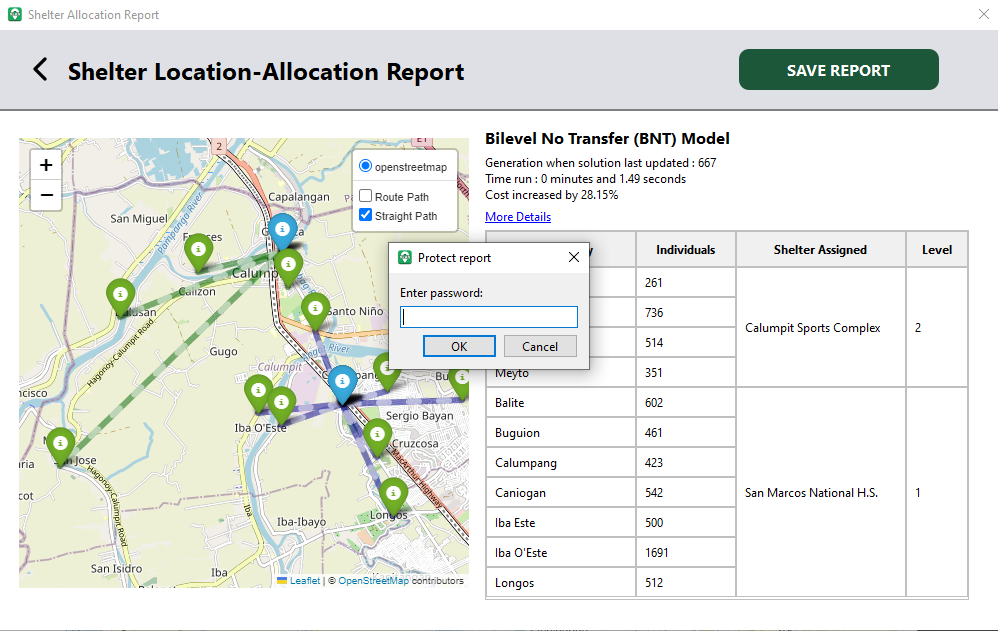
\includegraphics[width=0.6\columnwidth]{Chapter 4/alloc report pass}
		\label{passPop}
	\end{figure}
	
	
	\subsection{Generated Shelter Location-Allocation Report}
	 Table \ref{calReport} presents the optimized shelter location-allocation results generated by the system. Five shelters were opened and assigned to respective communities. All shelters were opened as Level 1, except for Mun. Covered Court, which was upgraded to Level 2. The data used considers only 12\% of the population in each barangay as affected based from \textcite{Opdyke2024}. Additionally, the shelters have a maintenance cost, which are factored into the optimization process. Table \ref{modelParams} shows the parameters used for the BNT model and the genetic algorithm.
	
	
	\begin{table}[H]
		\centering
		\caption{Generated Shelter Location-Allocation for Calumpit}
		\label{calReport}
		\renewcommand{\arraystretch}{1.1} 
		\resizebox{0.65\columnwidth}{!}{
			\begin{tabular}{|c|c|c|}
				\hline
				\textbf{Community} & \textbf{Shelter Assigned} & \textbf{Level} \\ \hline
				Calizon & \multirow{5}{*}{Doña Damiana Elem School} & \multirow{5}{*}{Level 1} \\ \cline {1-1} 
				Frances & & \\ \cline {1-1} 
				Gatbuca & & \\ \cline {1-1} 
				Meysulao & & \\ \cline {1-1} 
				San Miguel  & & \\ \hline
				
				Bulusan & \multirow{6}{*}{Mun. Covered Court} & \multirow{6}{*}{Level 2} \\ \cline {1-1} 
				Corazon & & \\ \cline {1-1} 
				Panducot & & \\ \cline {1-1} 
				Poblacion & & \\ \cline {1-1} 
				Santa Lucia & & \\ \cline {1-1} 
				Sucol & & \\ \hline
				
				Balungao & \multirow{5}{*}{NV9 Multi-Purpose} & \multirow{5}{*}{Level 1} \\ \cline {1-1} 
				Meyto & & \\ \cline {1-1} 
				San Jose & & \\ \cline {1-1} 
				Santo Niño & & \\ \cline {1-1} 
				Sapang Bayan & & \\ \hline
				
				Caniogan & \multirow{3}{*}{San Marcos Elem. Sch.} & \multirow{3}{*}{Level 1} \\ \cline {1-1} 
				Palimbang & & \\ \cline {1-1} 
				San Marcos & & \\ \hline
				
				Balite & \multirow{10}{*}{San Marcos National H.S.} & \multirow{10}{*}{Level 1} \\ \cline {1-1} 
				Baguion & & \\ \cline {1-1} 
				Calumpang & & \\ \cline {1-1} 
				Gugo & & \\ \cline {1-1} 
				Iba Este & & \\ \cline {1-1} 
				Iba O'Este & & \\ \cline {1-1} 
				Longos & & \\ \cline {1-1} 
				Pio Cruzcosa & & \\ \cline {1-1} 
				Pungo & & \\ \cline {1-1} 
				Sergio Bayan & & \\ \hline
			\end{tabular}
		}
		
	\end{table}
	
	
	\begin{table}[h]
		\centering
		\caption{Model Parameters}
		\label{modelParams}
		\begin{tabular}{|c|c|}
			\hline
			\textbf{Parameter} & \textbf{Value} \\ \hline
			Area Per Individual in $m^2$ & 1 \\ 
			Maximum Level 2 Shelters  & 33 \\ 
			Maximum Shelters & 33 \\ 
			Weight Distance & 0.5 \\ 
			Weight Cost & 0.5 \\ 
			Generations & 200000 \\ 
			Population & 100 \\ 
			Mutation Rate & 0.1 \\ \hline
		\end{tabular}
	\end{table}
	
	Table \ref{resdetails} shows the details of the result. Note that this report is generated by the system running on Huawei Matebook D15 with processor of Ryzen 7 5700U. The generated report can be downloaded as an Excel file. In the Report Module, a map displays where communities are allocated to their designated shelters. Figure \ref{straightpath} and \ref{routepath} shows the generated map which visualizes the allocation result.
	
	\begin{table}[h]
		\centering
		\caption{Result Details}
		\label{resdetails}
		\resizebox{0.8\columnwidth}{!}{
			\begin{tabular}{|p{7cm}|p{5cm}|}
				\hline
				\textbf{Item} & \textbf{Value} \\ \hline
				Objective Value & 72034087 \\ 
				Time Run  & 73 minutes and 30.96 seconds \\ 
				Cost of Opened Shelters & 144019600 \\ 
				Generation when solution last updated & 136256 \\ \hline
			\end{tabular}
		}
	\end{table}
	
	\begin{figure}[H]
		\centering
		\caption{Community to Shelter Paths}
		\begin{subfigure}{0.35\textwidth}
			\caption{Straight Path}
			\centering
			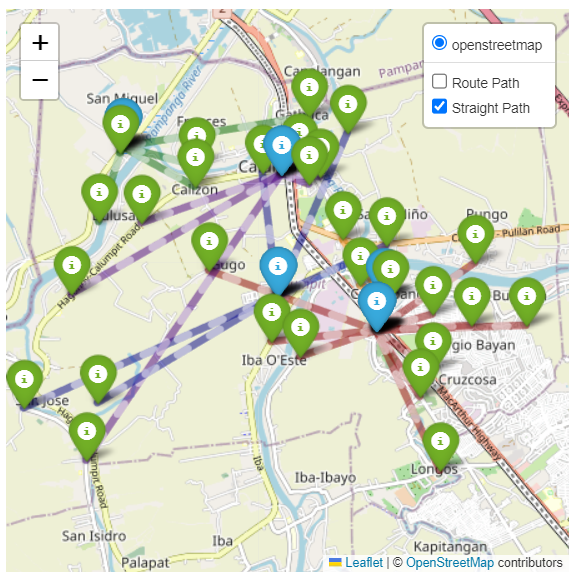
\includegraphics[width=\textwidth]{Chapter 4/straight path}
			\label{straightpath}
		\end{subfigure}
		\hspace{0.5cm}
		\begin{subfigure}{0.35\textwidth}
			\caption{Route Path}
			\centering
			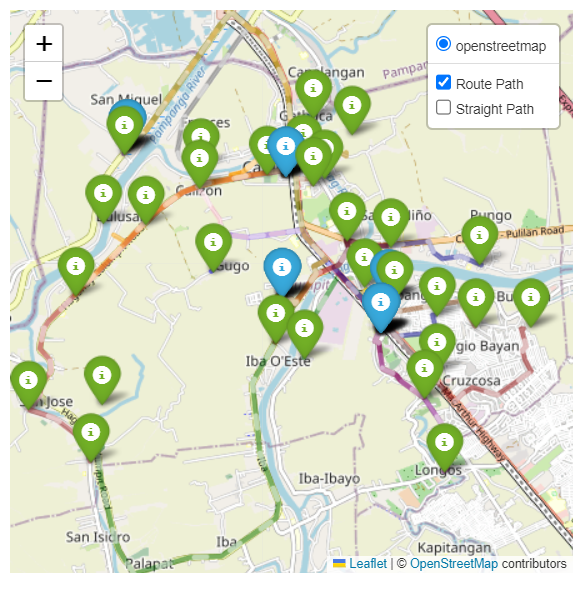
\includegraphics[width=\textwidth]{Chapter 4/route path}
			\label{routepath}
		\end{subfigure}
		
	\end{figure}
	
	
	\subsection{System Evaluation}
	The researchers conducted a survey to 23 respondents from the MSWDO and MDRRMO of Calumpit. The survey instrument was based on TAM which consists of four criteria: perceived usefulness, perceived ease of use, attitude towards using, and behavioral intention to use. The gathered data was analyzed to determine the users’ acceptance of the system. 
	
	\begin{table}[h!]
		\centering
		\caption{\textit{End User Evaluation}}
		\label{enduseeval}
		\renewcommand{\arraystretch}{1.3}
		\resizebox{0.8\columnwidth}{!}{
			\begin{tabular}{p{5cm}ccc}
				\hline
				\textbf{Criteria} & \textbf{Mean} & \textbf{SD Range} & \textbf{VI} \\
				\hline
				Perceived Usefulness 
				& 9.40 & 0.54-0.80 & Strongly Agree \\
				Perceived Ease of Use
				& 9.47& 0.58-0.66 & Strongly Agree \\
				Attitude Towards Using
				& 9.48 & 0.58-0.59 & Strongly Agree \\
				Behavioral Intention to Use
				& 9.41 & 0.58-0.70 & Strongly Agree \\
				\hline
			\end{tabular}
		}
	\end{table}
	
	Table \ref{enduseeval} presents the end-users' evaluation across the four determinants of TAM. The mean scores for all determinants range from 9.4 to 9.41, all interpreted as “Strongly Agree”. The standard deviations range from 0.54 to 0.8, indicating low variability in responses.
	
	To evaluate the system’s technical quality, the researchers surveyed five IT experts, from the faculty of the College of Information and Communications Technology (CICT) at Bulacan State University, and developers from a technology company. 
	
	\begin{table}[h!]
		\centering
		\caption{\textit{IT Experts Evaluation}}
		\label{itexpeval}
		\renewcommand{\arraystretch}{1.3}
		\resizebox{0.8\columnwidth}{!}{
			\begin{tabular}{p{5cm}ccc}
				\hline
				\textbf{Criteria} & \textbf{Mean} & \textbf{SD Range} & \textbf{VI} \\
				\hline
				Functional Suitability 
				& 9.80 & 0.00-0.55 & Strongly Agree \\
				Performance Efficiency
				& 9.67 & 0.45-0.55 & Strongly Agree \\
				Compatibility
				& 9.00 & 0.84-1.30 & Strongly Agree \\
				Interaction Capability
				& 9.33 & 0.45-0.84 & Strongly Agree \\
				Reliability
				& 9.60 & 0.45-0.71 & Strongly Agree \\
				Security
				& 9.67 & 0.45-1.30 & Strongly Agree \\
				Maintainability
				& 9.24 & 0.45-1.14 & Strongly Agree \\
				Flexibility
				& 9.50 & 0.00-1.10 & Strongly Agree \\
				\hline
			\end{tabular}
		}
	\end{table}
	
	Table \ref{itexpeval} presents the IT experts' evaluation across the eight criteria from ISO/IEC 25010. The mean scores for all determinants range from 9 to 9.8, all interpreted as “Strongly Agree”. The standard deviations range below 1.3, indicating low variability in responses.
	
	Feedback from IT experts recognized the system’s comprehensive functionality, reliable performance, and simple, user-friendly interface, effectively identifying optimal shelter locations and processing data efficiently. They recommended improvements such as supporting new model configurations without major code changes, enhancing the map layout, displaying additional details on user interaction, and strengthening data protection. Suggestions included developing a mobile app, adding travel time estimates, enabling real-time data updates, configuring models through the UI, and simplifying error messages for non-technical users. Meanwhile, LGU Calumpit officials stressed the importance of accurately identifying shelter lot locations. Overall, the feedback provides a clear guide for refining the system’s usability, adaptability, and effectiveness.
	

\section{Conclusion and Recommendations}
As the system was fully developed and the evaluation process was completed,
this chapter presents a summary of the key findings obtained, and
conclusions were drawn based on the results of the system evaluation.
	
	\subsection{Conclusion}
	The Shelter Location-Allocation System was developed for Calumpit, Bulacan to support disaster response planning by optimizing the assignment of communities to evacuation shelters. Using the Bilevel No Transfer Model integrated with a genetic algorithm, the system considers factors like distance, capacity, cost, and shelter levels. Key features include data and model modification, data simulation, shelter tagging, and report protection all contributing to an effective and quality decision support system for disaster response planning. 
	
	After running 200,000 generations in 73 minutes, the system identified five optimal shelters, with one required to be a level 2 shelter. This suggests that upgrading an existing shelter is more optimal than opening an additional one. It also indicates that other built shelters may remain closed to minimize maintenance costs. Additionally, no empty lots were selected, which may imply that constructing a new shelter is not yet necessary. However, it is important to note that actual affected population and cost considerations may differ based on the decision maker's assessments. The system allows users to adjust data and model parameters as needed. 
	
	Evaluation by LGU staff and IT experts rated the system highly in acceptability, functionality, and reliability, with both groups strongly agreeing on its usefulness. This suggests that they are likely to adopt and use the system to support their work in disaster response planning, while also confirming that it meets international standards for a software product.
	
	\subsection{Recommendations}
	Recommendations for future work include exploring additional shelter location models, integrating GIS and real-time data, testing in other municipalities, and improving cross-platform compatibility. Feedback also suggested enhancing data protection, model configurability, and adding mobile accessibility to better support evolving disaster response needs.
	
	
\printbibliography[heading=bibintoc,title={REFERENCES}] %<-start the bibliography
\end{document}